\documentclass{standalone}


\usepackage{tikz}
\usepackage{pgfplots}
\usetikzlibrary{calc}
\pgfplotsset{compat=1.15}

\begin{document}

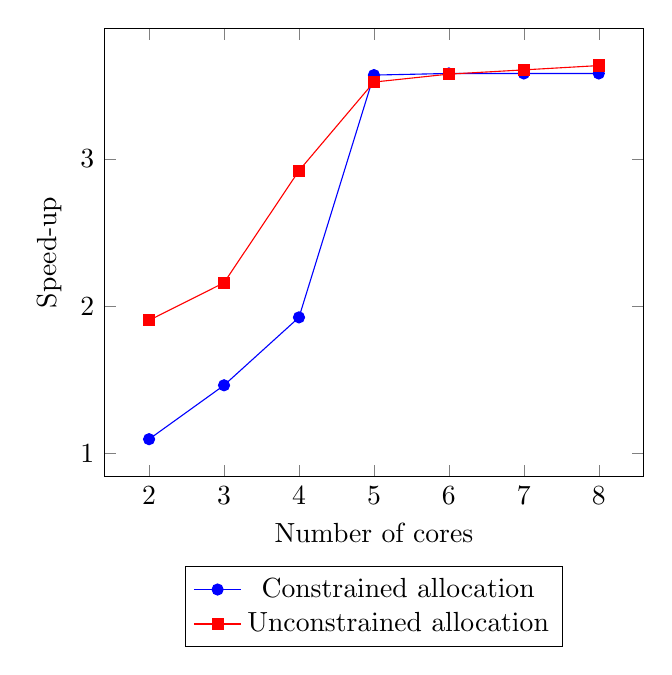
\begin{tikzpicture}
    \begin{axis}[
        xlabel=Number of cores,
        ylabel=Speed-up,legend style={at={(0.5,-0.2)},anchor=north}]
    \addplot[mark=*,blue,label=const] plot coordinates {
        (2,     1.097909998)
        (3,    1.463604418)
        (4,    1.924422442)
        (5,   3.568543452)
        (6,   3.579496624)
        (7,   3.579496624)
        (8,  3.579496624)
    };
    \addlegendentry{Constrained allocation}

    \addplot[color=red,mark=square*,label=unconst]
        plot coordinates {
        (2,     1.904310908)
        (3,    2.15962963)
        (4,   2.91987982)
        (5,   3.521135266)
        (6,  3.575107296)
        (7,  3.603831891)
        (8,  3.633021807)
        }; 
    \addlegendentry{Unconstrained allocation}
    \end{axis}
\end{tikzpicture}

\end{document}